\documentclass[12pt,a4paper]{article}

\usepackage[utf8]{inputenc}
\usepackage[T5]{fontenc}
\usepackage[vietnamese]{babel}
\usepackage{geometry}
\usepackage{graphicx}
\usepackage{booktabs}
\usepackage{array}
\usepackage{float}
\usepackage{xcolor}
\usepackage{hyperref}

\geometry{margin=2.2cm}
\graphicspath{{figures/ai_test_validation/}}
\hypersetup{colorlinks=true, linkcolor=blue, urlcolor=blue}

\title{\textbf{Báo cáo ngắn kiểm thử mô hình AI phân loại rác}}
\author{AIoT Smart Trash Bin}
\date{Ngày kiểm thử: 11/07/2026}

\begin{document}
\maketitle

\section{Mục tiêu}
Báo cáo này tổng hợp kết quả kiểm thử theo tài liệu
\texttt{docs/03\_TEST\_VALIDATION.md}. Phạm vi đã thực hiện gồm kiểm thử model
float và model INT8 trên máy tính. Các tầng kiểm thử ESP32, end-to-end servo,
độ trễ thực tế và độ bền hệ thống chưa được thực hiện trong lần chạy này.

\section{Dữ liệu và artifact}
Model được train chỉ với hai lớp \texttt{paper} và \texttt{plastic}. Các ảnh
khác trong TrashNet chỉ dùng cho hiệu chỉnh và kiểm thử cơ chế từ chối
\texttt{OTHER}, không dùng để cập nhật trọng số CNN.

\begin{table}[H]
\centering
\caption{Thống kê tập dữ liệu dùng trong lần kiểm thử}
\begin{tabular}{lrrr}
\toprule
\textbf{Split} & \textbf{Paper} & \textbf{Plastic} & \textbf{Other} \\
\midrule
Train known & 403 & 347 & -- \\
Validation known/other & 83 & 61 & 184 \\
Test known/other & 108 & 74 & 249 \\
\bottomrule
\end{tabular}
\end{table}

Artifact chính sau khi export:
\texttt{model\_float.keras},
\texttt{model\_int8.tflite},
\texttt{model\_data.cc},
\texttt{model\_data.h},
\texttt{labels.json},
\texttt{thresholds.json},
\texttt{centroids.json},
\texttt{quantization.json},
\texttt{metrics\_float\_eval.json} và
\texttt{metrics\_int8.json}.

\section{Kết quả phân loại paper/plastic}
Bảng sau chỉ xét hai lớp đã train, chưa tính cơ chế từ chối \texttt{OTHER}.
Mục tiêu recall cho từng lớp là tối thiểu 85\%.

\begin{table}[H]
\centering
\caption{Kết quả test hai lớp đã train}
\begin{tabular}{lrrrr}
\toprule
\textbf{Model} & \textbf{Accuracy} & \textbf{Macro F1} &
\textbf{Recall paper} & \textbf{Recall plastic} \\
\midrule
Tiny CNN float & 87.91\% & 87.53\% & 88.89\% & 86.49\% \\
Tiny CNN INT8 & 87.36\% & 86.99\% & 87.96\% & 86.49\% \\
\bottomrule
\end{tabular}
\end{table}

\begin{figure}[H]
\centering
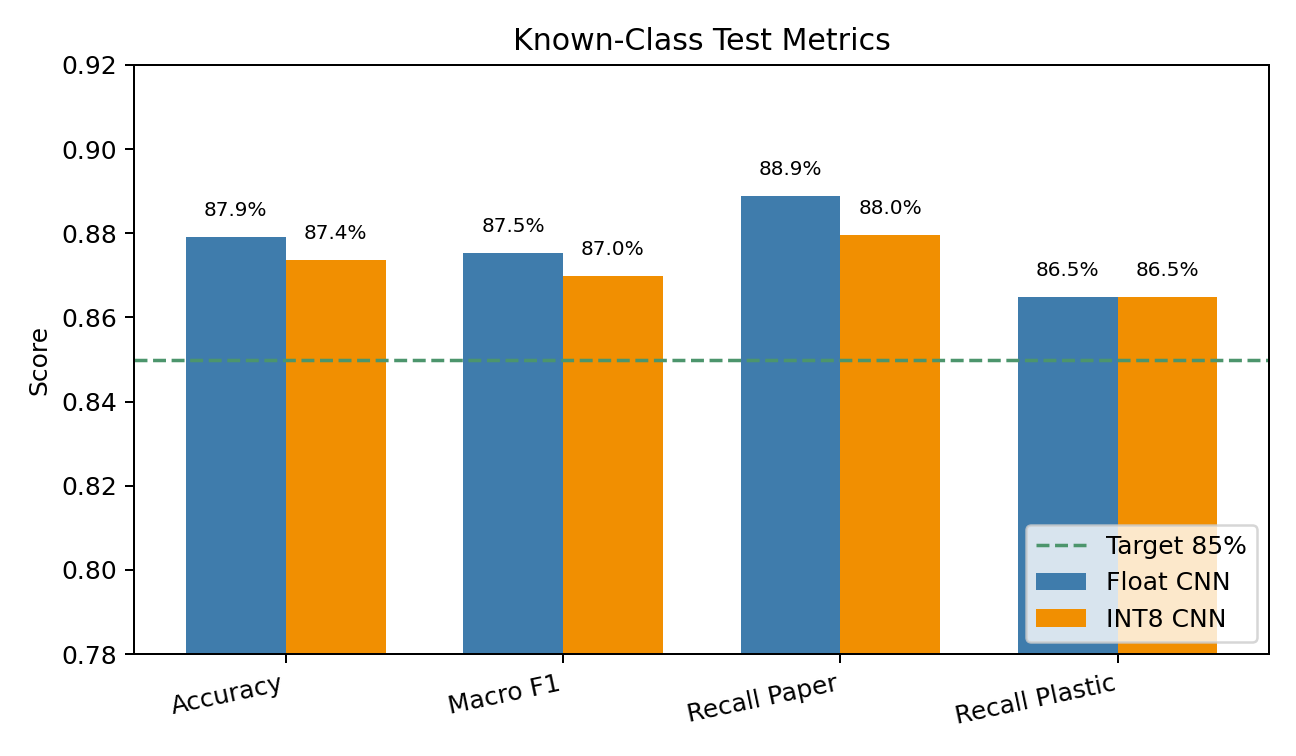
\includegraphics[width=0.92\linewidth]{known_metric_comparison.png}
\caption{So sánh các chỉ số trên tập test paper/plastic giữa model float và INT8.}
\end{figure}

Kết quả cho thấy quá trình lượng tử hóa INT8 không làm giảm chất lượng đáng kể:
accuracy giảm khoảng 0.55 điểm phần trăm, recall plastic giữ nguyên và recall
paper giảm nhẹ.

\section{Kết quả ba đầu ra với OTHER}
Khi áp dụng ngưỡng \texttt{confidence}, \texttt{margin} và khoảng cách centroid
để sinh nhãn \texttt{OTHER}, kết quả trên tập test ba đầu ra như sau.

\begin{table}[H]
\centering
\caption{Kết quả ba đầu ra sau khi bật cơ chế từ chối}
\begin{tabular}{lrrrrr}
\toprule
\textbf{Model} & \textbf{Accuracy} & \textbf{Macro F1} &
\textbf{Recall paper} & \textbf{Recall plastic} &
\textbf{Other false accept} \\
\midrule
Tiny CNN float & 39.68\% & 39.18\% & 88.89\% & 82.43\% & 94.38\% \\
Tiny CNN INT8 & 39.68\% & 39.42\% & 87.96\% & 82.43\% & 93.98\% \\
\bottomrule
\end{tabular}
\end{table}

\begin{table}[H]
\centering
\caption{Confusion matrix INT8 sau rejection}
\begin{tabular}{lrrr}
\toprule
\textbf{Thực tế / Dự đoán} & \textbf{PAPER} & \textbf{PLASTIC} & \textbf{OTHER} \\
\midrule
PAPER & 95 & 12 & 1 \\
PLASTIC & 10 & 61 & 3 \\
OTHER & 64 & 170 & 15 \\
\bottomrule
\end{tabular}
\end{table}

\begin{figure}[H]
\centering
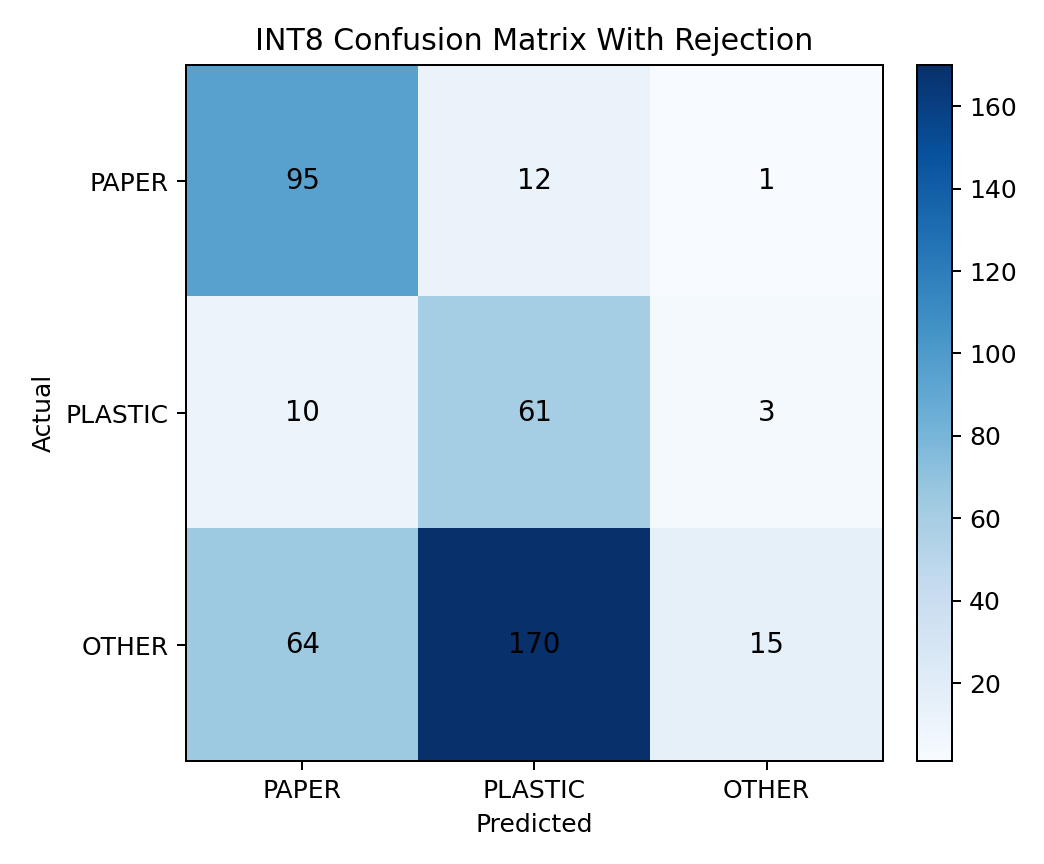
\includegraphics[width=0.72\linewidth]{int8_confusion_matrix.png}
\caption{Heatmap confusion matrix của model INT8 khi có cơ chế rejection.}
\end{figure}

Kết quả \texttt{OTHER} chưa đạt yêu cầu nghiệm thu. Mục tiêu trong tài liệu là
\texttt{OTHER false accept} không quá 10\%, trong khi kết quả hiện tại là
93.98\% với model INT8. Nguyên nhân chính là các ảnh \texttt{cardboard},
\texttt{glass}, \texttt{metal}, \texttt{trash} của TrashNet có phân bố
confidence và embedding chồng mạnh với hai lớp paper/plastic.

\section{Ảnh minh chứng}
\begin{figure}[H]
\centering
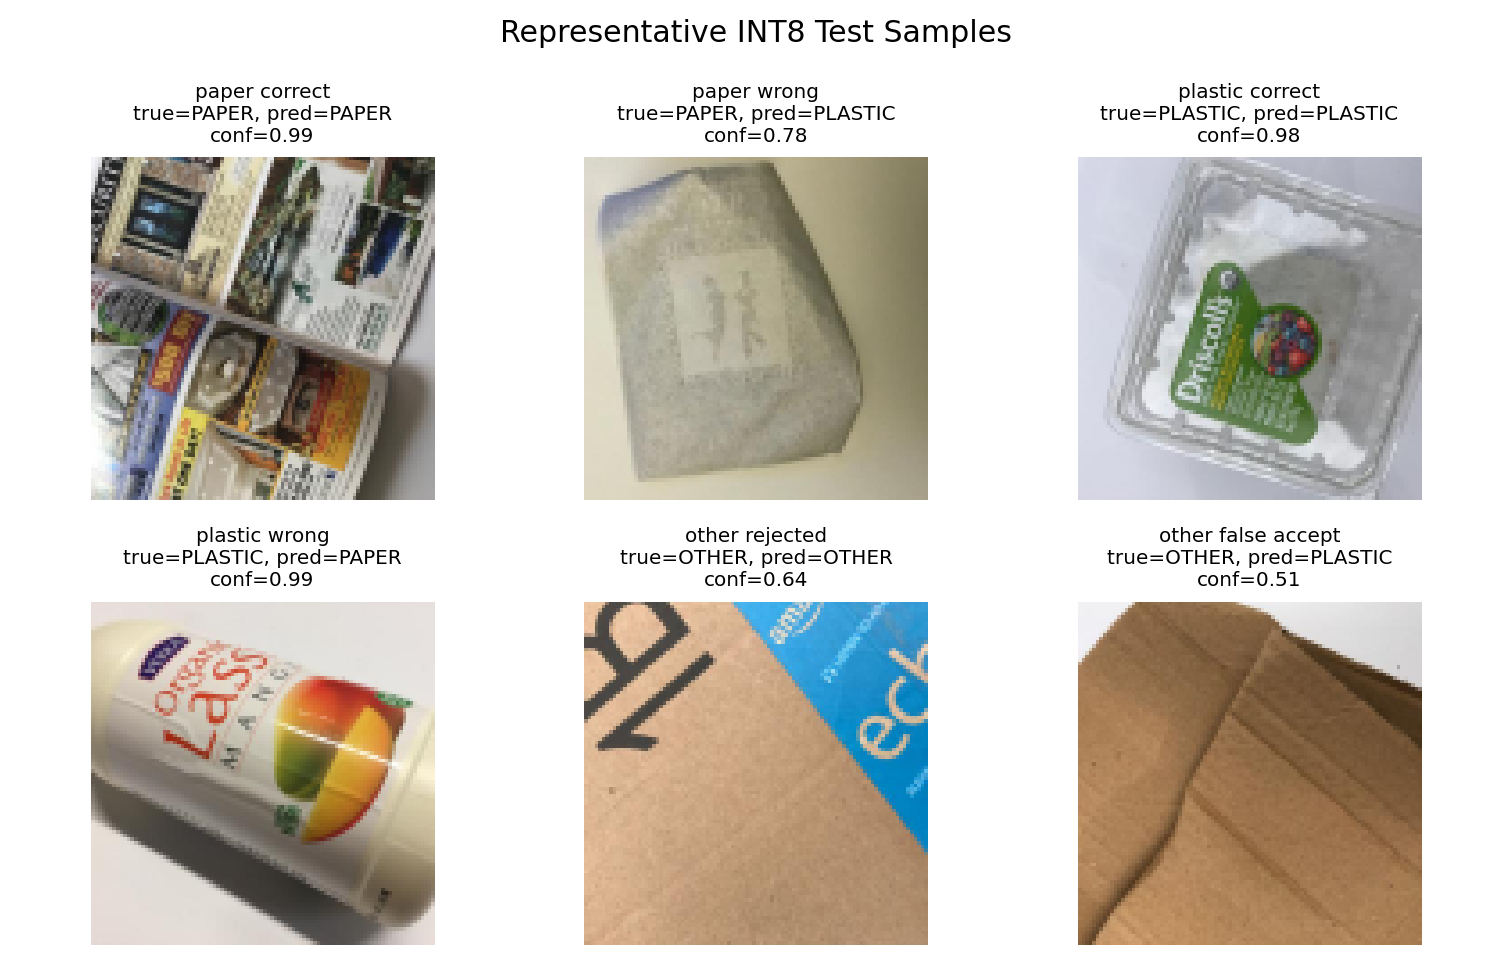
\includegraphics[width=0.95\linewidth]{int8_test_samples.png}
\caption{Một số ảnh test đại diện, gồm mẫu dự đoán đúng, mẫu sai và mẫu
\texttt{OTHER} bị false accept.}
\end{figure}

\section{Bảng test theo yêu cầu validation}
\begin{table}[H]
\centering
\caption{Bảng test case tóm tắt}
\begin{tabular}{>{\raggedright\arraybackslash}p{2.8cm}
                >{\raggedright\arraybackslash}p{6.4cm}
                >{\raggedright\arraybackslash}p{3.2cm}}
\toprule
\textbf{ID} & \textbf{Nội dung kiểm thử} & \textbf{Kết quả} \\
\midrule
AI-PC-01 & Kiểm tra model float trên tập test paper/plastic. &
\textcolor{green!45!black}{Đạt}: accuracy 87.91\%. \\
AI-PC-02 & Kiểm tra model INT8 trên tập test paper/plastic. &
\textcolor{green!45!black}{Đạt}: accuracy 87.36\%. \\
AI-PC-03 & Kiểm tra recall từng lớp của model INT8. &
\textcolor{green!45!black}{Đạt}: paper 87.96\%, plastic 86.49\%. \\
AI-OTHER-01 & Kiểm tra false accept của lớp OTHER trên INT8. &
\textcolor{red!70!black}{Chưa đạt}: 93.98\%. \\
QT-01 & Kiểm tra full integer quantization. &
\textcolor{green!45!black}{Đạt}: input/output INT8. \\
FW-ESP32-01 & So khớp Python INT8 và ESP32. &
Chưa thực hiện. \\
E2E-01 & Test mở đúng ba cổng servo trong tối đa 5 giây. &
Chưa thực hiện. \\
STAB-01 & Test độ bền tối thiểu 100 chu kỳ. &
Chưa thực hiện. \\
\bottomrule
\end{tabular}
\end{table}

\section{Kết luận}
Model Tiny CNN INT8 đã đạt mục tiêu phân biệt hai lớp \texttt{paper} và
\texttt{plastic} trên tập test hiện tại. Tuy nhiên, hệ thống chưa đạt nghiệm thu
AI ba đầu ra vì cơ chế \texttt{OTHER} còn false accept quá cao. Cần bổ sung tập
\texttt{validation\_other/other} và \texttt{test/other} được chụp bằng prototype
thực tế, sau đó calibrate lại threshold và chạy tiếp kiểm thử ESP32, servo,
độ trễ và độ bền.

\end{document}
